\documentclass[tikz,border=7pt]{standalone}
\usepackage{pgfplots}
\pgfplotsset{compat=1.18}
\begin{document}
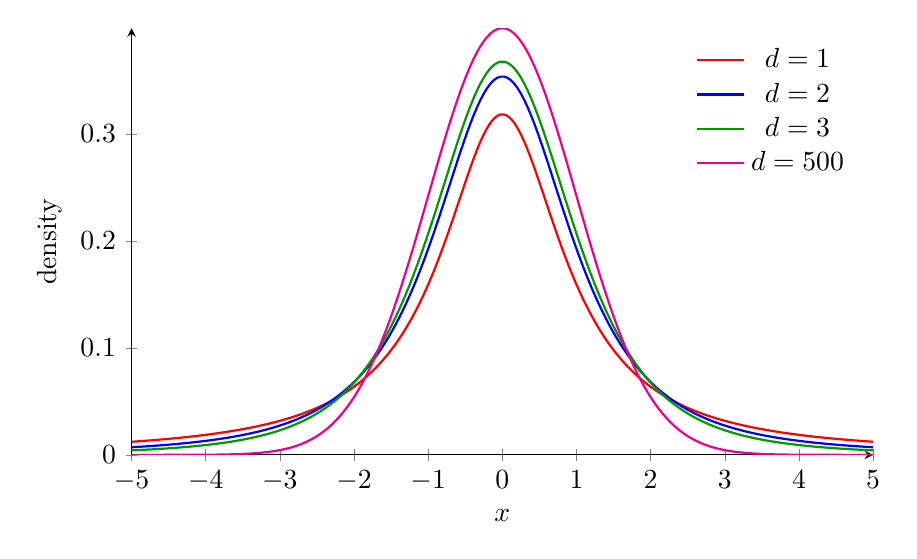
\begin{tikzpicture}
\begin{axis}[width=11cm,height=7cm,axis lines=left,xmin=-5,xmax=5,ymin=0,samples=220,xlabel={$x$},ylabel={density},legend style={draw=none}]
\addplot[red,thick,domain=-5:5] {1/(pi*(1+x^2))}; \addlegendentry{$d=1$}
\addplot[blue,thick,domain=-5:5] {.353553*(1+x^2/2)^(-1.5)}; \addlegendentry{$d=2$}
\addplot[green!60!black,thick,domain=-5:5] {.367553*(1+x^2/3)^(-2)}; \addlegendentry{$d=3$}
\addplot[magenta,thick,domain=-5:5] {.39874*exp(-x^2/2)}; \addlegendentry{$d=500$}
\end{axis}
\end{tikzpicture}
\end{document}
